\documentclass[noamssymb,svgnames]{beamer}
\usecolortheme{beaver}
\usefonttheme{serif}
\usefonttheme{professionalfonts}

\usepackage[bitstream-charter]{mathdesign} % Use BT Charter font
\usepackage{beramono}                      % Use Vera Mono for \ttfamily
\usepackage[T1]{fontenc}                   % Use T1 encoding instead of OT1
\usepackage[utf8]{inputenc}                % Use UTF8 input encoding
\usepackage{microtype}                     % Improve typography
\usepackage{booktabs}
\usepackage[binary-units]{siunitx}
\usepackage{tikz}
\usetikzlibrary{shapes.geometric}

\usepackage{hyperref}
\hypersetup{pdfstartview=Fit}

% BEAMER CONFIGURATION ---------------------------------------------------------
\setbeamerfont{block title}{size=\normalsize}
\setbeamerfont{block body}{size=\scriptsize}
\setbeamercolor{block title}{fg=darkred,bg=gray!10!white}
\setbeamercolor*{item}{fg=darkred}

% TCOLORBOX / MINTED CONFIGURATION ---------------------------------------------
\usepackage[many,minted]{tcolorbox}
\NewTCBListing{python}{ O{} }{listing only,minted language=python,#1}
\NewTCBListing{shell}{ O{} }{%
  listing only,minted language=shell,%
  minted options={fontsize=\footnotesize},#1}
\tcbset{listing only}
\setminted{
  mathescape,
  autogobble,
  fontfamily=courier,
  framesep=2mm
}

\definecolor{darkblue}{rgb}{0.0,0.0,0.6}
\newcommand{\obj}[1]{\texttt{\color{darkblue}#1}}

% ------------------------------------------------------------------------------
\title{Running in Parallel}

\institute{
\includegraphics[width=2in]{../images/openmc_logo.png}}

\date{OpenMC Workshop \\ Canadian Nuclear Laboratories \\ March 14--16, 2017}

% ------------------------------------------------------------------------------
\begin{document}

\frame{\titlepage}

% ------------------------------------------------------------------------------

\begin{frame}{Parallelism in OpenMC}
  \begin{itemize}
  \item OpenMC is capable of using both distributed-memory (MPI) and
    shared-memory (OpenMP) parallelism
  \item On a single node machine (workstation, laptop, etc.), your best bet is
    probably to use OpenMP
  \item On a cluster/supercomputer, you will probably want to use MPI or
    MPI+OpenMP
  \end{itemize}
\end{frame}

\begin{frame}[fragile]{OpenMP}
  \begin{itemize}
  \item Create multiple threads, each of which can simulate its own particle
  \item If you have $T$ cores, can attain $T$ times speedup at best
  \item In practice, you probably won't get $T$:
    \begin{itemize}
    \item Shared hardware resources
    \item Cache misses due to eviction
    \end{itemize}
  \item Using OpenMP consumes very little extra memory!
  \end{itemize}
  \vfill
  To use OpenMP:
  \begin{shell}
    cmake -Dopenmp=on ..
    make
  \end{shell}
\end{frame}

\begin{frame}{Message Passing Interface (MPI)}
  \begin{itemize}
  \item MPI defines a library specification for message-passing between
    processes
  \item Two major implementations: OpenMPI and MPICH
  \item With $N$ nodes, usually get can $N$ speedup
  \item When using MPI, entire memory space is replicated for each process
    \begin{itemize}
      \item If your model requires \SI{1}{\giga\byte} of tallies and you run it
        on 32 processes, you need at least \SI{32}{\giga\byte} of memory
    \end{itemize}
  \end{itemize}
\end{frame}

\begin{frame}[fragile]{Running with MPI}
  \begin{enumerate}
  \item Install MPICH/OpenMPI, e.g., on Debian derivatives
  \begin{shell}
    sudo apt install mpich libmpich-dev
    sudo apt install openmpi-bin libopenmpi-dev
  \end{shell}
  \item When compiling OpenMP, need to specify MPI compiler wrappers.
    \begin{shell}
      export FC=mpifort
      export CC=mpicc
      export CXX=mpicxx
      cmake ..
      make
    \end{shell}
  \end{enumerate}
\end{frame}

\begin{frame}[fragile]{Specifying threads/processes}
  From the command line:
  \begin{shell}
    openmc -s 8
    mpiexec -n 32 openmc
    mpiexec -n 4 openmc -s 8
  \end{shell}
  \vfill
  Or from Python directly:
  \begin{python}[minted options={fontsize=\scriptsize}]
    openmc.run(threads=8)
    openmc.run(mpi_args=['mpiexec', '-n', '32'])
    openmc.run(threads=8, mpi_args=['mpiexec', '-n', '32'])
  \end{python}
  \vfill
  For OpenMP, can also set environment variable
  \begin{shell}
    export OMP_NUM_THREADS=8
  \end{shell}
\end{frame}

\begin{frame}{General Advice}
  \begin{itemize}
  \item Use OpenMP within each NUMA node
  \item Make sure number of particles per generation is large enough (reduces
    relative time for fission bank and tally synchronization)
  \item Use hardware threading if available (e.g., Intel hyperthreading)
  \item Use process binding
  \end{itemize}
\end{frame}

\begin{frame}{Xeon Haswell-EP}
  \begin{center}
    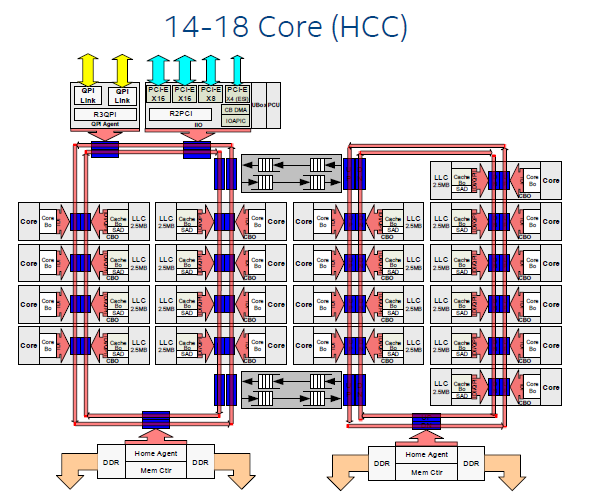
\includegraphics[width=0.8\textwidth]{../images/HaswellEP_DieConfig.png}
  \end{center}
\end{frame}

\begin{frame}{Xeon Phi KNL}
  \begin{center}
    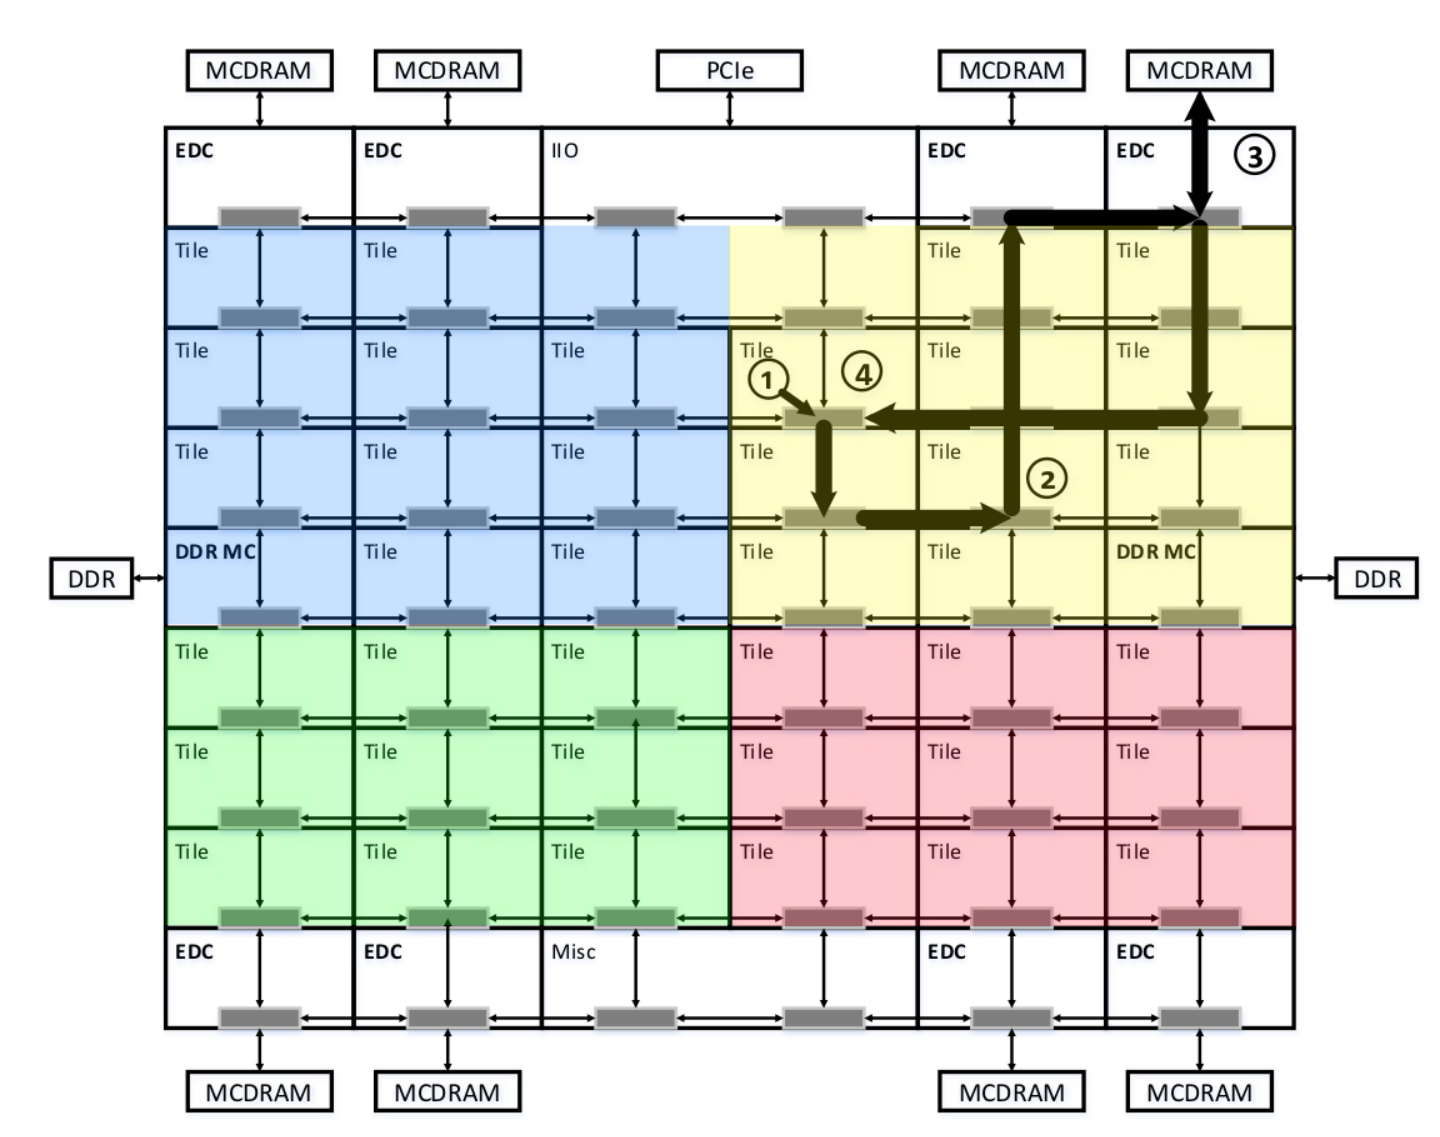
\includegraphics[width=0.8\textwidth]{../images/XeonPhiKNL.png}
  \end{center}
\end{frame}

\begin{frame}[fragile]{Process Binding}
  Binding Options:
  \begin{itemize}
  \item \obj{hwthread}, \obj{core}, \obj{l1cache}, \obj{l2cache}, \obj{l3cache},
    \obj{socket}, \obj{numa}, \obj{board}
  \end{itemize}
  \vfill
  MPICH:
  \begin{shell}[minted options={fontsize=\scriptsize}]
    mpiexec -bind-to socket ...
  \end{shell}
  \vfill
  OpenMPI:
  \begin{shell}
    mpiexec --bind-to socket ...
  \end{shell}
\end{frame}

\end{document}
